% This is the Reed College LaTeX thesis template. Most of the work
% for the document class was done by Sam Noble (SN), as well as this
% template. Later comments etc. by Ben Salzberg (BTS). Additional
% restructuring and APA support by Jess Youngberg (JY).
% Your comments and suggestions are more than welcome; please email
% them to cus@reed.edu
%
% See https://www.reed.edu/cis/help/LaTeX/index.html for help. There are a
% great bunch of help pages there, with notes on
% getting started, bibtex, etc. Go there and read it if you're not
% already familiar with LaTeX.
%
% Any line that starts with a percent symbol is a comment.
% They won't show up in the document, and are useful for notes
% to yourself and explaining commands.
% Commenting also removes a line from the document;
% very handy for troubleshooting problems. -BTS

% As far as I know, this follows the requirements laid out in
% the 2002-2003 Senior Handbook. Ask a librarian to check the
% document before binding. -SN

%%
%% Preamble
%%
% \documentclass{<something>} must begin each LaTeX document
\documentclass[12pt,twoside]{templates/facsothesis}
% Packages are extensions to the basic LaTeX functions. Whatever you
% want to typeset, there is probably a package out there for it.
% Chemistry (chemtex), screenplays, you name it.
% Check out CTAN to see: https://www.ctan.org/
%%
\ifxetex
  \usepackage{polyglossia}
  \setmainlanguage{spanish}
  % Tabla en lugar de cuadro
  \gappto\captionsspanish{\renewcommand{\tablename}{Tabla}
          \renewcommand{\listtablename}{Índice de tablas}}
\else
  \usepackage[spanish,es-tabla]{babel}
\fi
%\usepackage[spanish]{babel}
\usepackage{graphicx,latexsym}
\usepackage{amsmath}
\usepackage{amssymb,amsthm}
\usepackage{longtable,booktabs,setspace}
\usepackage{chemarr} %% Useful for one reaction arrow, useless if you're not a chem major
\usepackage[hyphens]{url}
% Added by CII
%\usepackage{hyperref}
\usepackage[colorlinks = true,
            linkcolor = blue,
            urlcolor  = blue,
            citecolor = blue,
            anchorcolor = blue]{hyperref}
\usepackage{lmodern}
\usepackage{float}
\floatplacement{figure}{H}
% End of CII addition
\usepackage{rotating}
\usepackage{placeins} % para fijar la posición de las tablas con \FloatBarrier


\usepackage[]{natbib}


% Next line commented out by CII
%\usepackage{biblatex}
%\usepackage{natbib}
% Comment out the natbib line above and uncomment the following two lines to use the new
% biblatex-chicago style, for Chicago A. Also make some changes at the end where the
% bibliography is included.
%\usepackage{biblatex-chicago}
%\bibliography{thesis}


% Added by CII (Thanks, Hadley!)
% Use ref for internal links
\renewcommand{\hyperref}[2][???]{\autoref{#1}}
\def\chapterautorefname{Chapter}
\def\sectionautorefname{Section}
\def\subsectionautorefname{Subsection}
% End of CII addition

% Added by CII
\usepackage{caption}
\captionsetup{width=5in}
% End of CII addition

% \usepackage{times} % other fonts are available like times, bookman, charter, palatino

% Syntax highlighting #22

% To pass between YAML and LaTeX the dollar signs are added by CII
\title{Confianza política, percepción del desempeño y confianza generalizada: un estudio empírico para el caso chileno}
\author{Juan Pablo Díaz}
% The month and year that you submit your FINAL draft TO THE LIBRARY (May or December)
\date{2025-10-14}
\division{}
\advisor{Profesor/a guía: Juan Carlos Castillo}
\institution{Universidad de Chile}
\degree{Seminario / Memoria / Tesis de Grado - Carrera de Sociología}
%If you have two advisors for some reason, you can use the following
% Uncommented out by CII
% End of CII addition

%%% Remember to use the correct department!
\department{}
% if you're writing a thesis in an interdisciplinary major,
% uncomment the line below and change the text as appropriate.
% check the Senior Handbook if unsure.
%\thedivisionof{The Established Interdisciplinary Committee for}
% if you want the approval page to say "Approved for the Committee",
% uncomment the next line
%\approvedforthe{Committee}

% Added by CII
%%% Copied from knitr
%% maxwidth is the original width if it's less than linewidth
%% otherwise use linewidth (to make sure the graphics do not exceed the margin)
\makeatletter
\def\maxwidth{ %
  \ifdim\Gin@nat@width>\linewidth
    \linewidth
  \else
    \Gin@nat@width
  \fi
}
\makeatother

%Added by @MyKo101, code provided by @GerbrichFerdinands

\setlength\parindent{0pt}


% Added by CII

\providecommand{\tightlist}{%
  \setlength{\itemsep}{0pt}\setlength{\parskip}{0pt}}

\Acknowledgements{

}

\Dedication{

}

\Preface{

}

\Abstract{

}

	\usepackage{booktabs}
\usepackage{longtable}
\usepackage{array}
\usepackage{multirow}
\usepackage{wrapfig}
\usepackage{float}
\usepackage{colortbl}
\usepackage{pdflscape}
\usepackage{tabu}
\usepackage{threeparttable}
\usepackage{threeparttablex}
\usepackage[normalem]{ulem}
\usepackage{makecell}
\usepackage{xcolor}
% End of CII addition
%%
%% End Preamble
%%
%
\let\chaptername\relax
\begin{document}
\bibliographystyle{apalike}
% Everything below added by CII
  \maketitle

\frontmatter % this stuff will be roman-numbered
\pagestyle{empty} % this removes page numbers from the frontmatter



%  \hypersetup{linkcolor=black}
  \setcounter{tocdepth}{1}
  \setlength{\parskip}{0pt}
  \tableofcontents

\setlength\parskip{1em plus 0.1em minus 0.2em}

  \listoftables

  \listoffigures



\mainmatter % here the regular arabic numbering starts
\pagestyle{fancyplain} % turns page numbering back on

\chapter*{Resumen}\label{resumen}
\addcontentsline{toc}{chapter}{Resumen}

Pendiente

\chapter*{Agradecimientos}\label{agradecimientos}
\addcontentsline{toc}{chapter}{Agradecimientos}

Pendiente

\chapter{Introducción}\label{introducciuxf3n}

A lo largo del tiempo, la comunidad científica ha destacado la importancia que tiene la confianza política para la estabilidad y el buen funcionamiento de los regímenes democráticos \citep{zmerliPoliticalTrust2022}. Desde el punto de vista de las instituciones, se argumenta que cuando estas son percibidas como confiables, ostentan una mayor efectividad en la implementación de servicios públicos, facilitan el consenso de los perdedores electorales, reducen la evasión fiscal y poseen una mayor resistencia a periodos de crisis económicas y sociales \citep{vandermeerDeeplyRootedConcern2017, newtonSocialPoliticalTrust2017, citrinPoliticalTrustCynical2018}. A su vez, se plantea que los ciudadanos que confían en sus instituciones tendrían una mayor tendencia a obedecer la ley, a interesarse en política y a respaldar políticas públicas que impliquen un riesgo o sacrificio personal \citep{citrinPoliticalTrustCynical2018, zmerliPoliticalTrust2022}. Por el contrario, se asume comúnmente que los ciudadanos que no confían en sus instituciones políticas serían más propensos a radicalizarse y a impulsar cambios que podrían significar a largo plazo un peligro para la supervivencia de la democracia \citep{andersonSensitiveLeftImpervious2008}. En este sentido, la confianza política se concibe como una condición previa para la consolidación de un régimen democrático \citep{vandermeerDeeplyRootedConcern2017}.

Según datos del PNUD \citeyearpar{pnudDiezAnosAuditoria2019}, Chile evidencia durante el periodo 2008-2018 una caída sostenida de la confianza que sus ciudadanos depositan en el gobierno, el Congreso, los tribunales de justicia y los partidos políticos. A su vez, durante este periodo se diluyeron las diferencias que al principio había en la confianza en las instituciones políticas según edad, nivel educacional, identificación con el eje izquierda y derecha, y pertenencia a zonas urbanas o rurales. Al situar estos datos a nivel regional, se evidencia que las instituciones chilenas tienen un nivel de confianza similar al del resto de países de la región, sin embargo, al extender el radio de comparación hacia el conjunto de países miembros de la OCDE, se ve que Chile es el cuarto país en el que más ha disminuido la confianza política para este periodo \citep{pnudDiezAnosAuditoria2019}. En paralelo a lo anterior, a lo largo de estos años aparecieron distintos movimientos sociales y ciclos de movilizaciones en los cuales se manifestaba un rechazo explícito a la institucionalidad política \citep{avendanoPropuestasCambioDebilidad2021, barozetEntreUrnaRedes2016}. Lo anterior, sumado al fracaso de los intentos de encausar institucionalmente esta crisis mediante la creación de una nueva constitución, dan cuenta de que el país vive una crisis de confianza en sus instituciones políticas que a día de hoy sigue sin resolución. Al alero de las consideraciones sobre la importancia que la literatura atribuye a la confianza política para la estabilidad y permanencia en el tiempo de los regímenes democráticos, se afirma la necesidad de investigar empíricamente algunos de los factores que podrían estar contribuyendo a esta crisis de confianza.

Esta necesidad ya ha sido abordada por otros investigadores con anterioridad \citep[véase][]{bargstedSocialPoliticalTrust2023, moralesquirogaEvaluandoConfianzaInstitucional2008, riffoQueInfluyeConfianza2019, saldanazunigaConfianzaInstitucionesPoliticas2019, segoviaMalaiseDemocracyChile2016, segoviaConfianzaInstitucionesPoliticas2008}, sin embargo, se identifican en estos estudios algunos vacíos que buscarán ser llenados por la presente investigación. En primer lugar, se observa una brecha temporal, en cuanto la mayoría de los estudios mencionados (a excepción de Bargsted et al. \citeyearpar{bargstedSocialPoliticalTrust2023}) se construyen sobre datos levantados con anterioridad al 2019. A lo largo de este periodo de tiempo que va desde el 2019 a la fecha, han ocurrido un conjunto de hitos como el estallido social, la pandemia de covid-19 y el fracaso de los procesos constituyentes. Debido a la relevancia de estos fenómenos en la configuración del panorama sociopolítico nacional, es importante explorar la posibilidad de variaciones en la magnitud de las relaciones encontradas con anterioridad. En segundo lugar, se identifica un déficit local en el estudio de algunos posibles determinantes de la confianza política que podrían ser particularmente importantes para el caso chileno, como la percepción de la desigualdad de ingresos, la corrupción y la confianza interpersonal. La necesidad de estudiar la relación con estos indicadores se fundamenta, por un lado, en los altos niveles de desigualdad de ingresos que reporta el país (con un coeficiente de Gini de 0.43 según el Banco Mundial \citeyearpar{bancomundialIndicadoresDesarrolloMundial2023}) y, por otro lado, en el surgimiento de diversos casos de corrupción con gran impacto en el escenario político nacional \citep{avendanoPropuestasCambioDebilidad2021}. Respecto a la confianza generalizada, se destaca el bajo nivel de confianza en los otros que reporta la población chilena (menor al 15\% según datos del PNUD \citeyearpar{pnudInformeSobreDesarrollo2024}).

Con el objetivo de profundizar en la comprensión de este fenómeno, se propone investigar la relación que existe entre la percepción del desempeño institucional ---expresada a través de la evaluación de la situación económica nacional, la corrupción y la desigualdad de ingresos---, la confianza generalizada y la confianza que los individuos depositan en sus instituciones políticas. La literatura especializada, en su mayoría, ha abordado estas relaciones de forma directa y por separado, concluyendo que tanto la percepción del desempeño en estas áreas como la confianza generalizada se asocian con la confianza política, aunque el efecto de la primera tiende a ser más intenso que el de la segunda \citep{mainwaringStateDeficienciesParty2006, mattesSocialPoliticalTrust2018, morrisCorruptionTrustTheoretical2010, newtonSocialPoliticalTrust2017}.

No obstante, estas investigaciones presentan una limitación importante: conciben la relación entre confianza generalizada y confianza política como un vínculo \emph{exclusivamente} directo. Lo anterior supone que la confianza interpersonal se basaría en un cálculo racional derivado de la experiencia, el cual terminaría por proyectarse de manera directa sobre las instituciones políticas. En contraste, siguiendo a Uslaner \citetext{\citeyear{uslanerMoralFoundationsTrust2002}; \citeyear{uslanerStudyTrust2017}}, se sostiene que este tipo de confianza refleja más bien una disposición moral a confiar en los otros, fundamentada en la percepción de que forman parte de una misma comunidad moral, y no en consideraciones estratégicas. Bajo esta perspectiva, se afirma la necesidad de ir más allá del estudio de la relación directa entre estos dos fenómenos. Para esto, se propone complementar este análisis con uno que indague en la posibilidad de que la confianza generalizada modere la relación entre la percepción del desempeño institucional y la confianza política, en cuanto los ciudadanos que confían en los demás serían menos susceptibles a disminuir su confianza en las instituciones políticas en función de malos desempeños.

Al alero de esta problematización, el presente estudio buscará analizar el impacto que tanto la percepción del desempeño institucional como la confianza generalizada tienen sobre la confianza política. A su vez, se pretende explorar posibles variaciones en la relación entre la percepción del desempeño institucional y la confianza política según el nivel de confianza generalizada presente en cada uno de los individuos. Para esto, se aplicará un modelo de regresión lineal con Mínimos Cuadrados Ordinarios (MCO) sobre datos extraídos de la encuesta Latinobarómetro en su versión del 2023. De esta forma, se buscará estimar la intensidad y significancia estadística de cada una de las relaciones planteadas, a modo de contrastar las hipótesis que guiarán esta investigación.

A continuación se presentará un apartado con la pregunta de investigación y los objetivos que guiarán esta investigación. Luego, se discutirán los conceptos principales y las hipótesis que se buscarán contrastar. Por último, se detallará la metodología a utilizar.

\section{Pregunta de investigación}\label{pregunta-de-investigaciuxf3n}

¿Cómo influyen la percepción del desempeño institucional y la confianza generalizada en la confianza política de los ciudadanos chilenos?

\section{Objetivo general}\label{objetivo-general}

Analizar la influencia que la percepción del desempeño institucional y la confianza generalizada tienen en la confianza política de los ciudadanos chilenos.

\section{Objetivos específicos}\label{objetivos-especuxedficos}

\begin{enumerate}
\def\labelenumi{\arabic{enumi}.}
\tightlist
\item
  Analizar el rol de la percepción del desempeño institucional en la confianza política de los ciudadanos chilenos.
\item
  Examinar el rol de la confianza generalizada en la confianza política de los ciudadanos chilenos.
\item
  Explorar si varía o no la relación entre la percepción del desempeño institucional y la confianza política al moderar por el nivel de confianza generalizada de los ciudadanos chilenos.
\end{enumerate}

\chapter{Antecedentes conceptuales y empíricos}\label{antecedentes-conceptuales-y-empuxedricos}

\section{Confianza política}\label{confianza-poluxedtica}

La confianza política se define como ``la expectativa de que las instituciones políticas funcionen según reglas justas incluso en ausencia de escrutinio constante''\footnote{Traducción propia.} \citep[p.16]{marienMeasuringPoliticalTrust2013}. En este sentido, esta categoría forma parte del más abarcador concepto de apoyo político acuñado por Easton \citetext{\citeyear{eastonSystemsAnalysisPolitical1965}; \citeyear{eastonReassessmentConceptPolitical1975}}. Este último, refiere a la forma en que un individuo se orienta evaluativamente hacia los componentes del sistema político, ya sea mediante sus actitudes o su comportamiento \citep{eastonReassessmentConceptPolitical1975}. A su vez, el autor divide los componentes del sistema político en tres: las autoridades en ejercicio, el régimen político y la comunidad política. De esta forma, el apoyo político se entiende como un \emph{continuum} que va desde el apoyo específico, orientado hacia las autoridades en función de la evaluación de su desempeño, hasta el apoyo difuso, dirigido hacia los principios y valores que subyacen al sistema político y a la comunidad que lo alberga \citep{eastonReassessmentConceptPolitical1975, norrisDemocraticDeficitCritical2011}. En este marco, la confianza política aparece como un indicador intermedio de apoyo, dirigido a las instituciones que forman parte del régimen político \citep{vandermeerDeeplyRootedConcern2017, zmerliPoliticalTrust2022}.

A su vez, la confianza política tiene sus fundamentos en un tipo específico de confianza estratégica que se puede resumir bajo la famosa fórmula ``A confía en B para que haga x''\footnote{Traducción propia.} \citep[p.26]{hardinWeWantTrust1999}. Esto implica que dicho concepto es relacional, en cuanto contempla un sujeto que confía y un objeto en quien se confía, y situacional, en cuanto refiere a cierto tipo de acción o contexto en el que se desenvuelve esta relación \citep{citrinPoliticalTrustCynical2018, vandermeerEconomicPerformancePolitical2018, vandermeerDeeplyRootedConcern2017}. En este sentido, entablar una relación de confianza implica un riesgo para el sujeto, el cual se encuentra en una relación de incertidumbre en torno al comportamiento que va a llevar a cabo el objeto en el que deposita su confianza. Es por esto que, desde el punto de vista de la confianza estratégica, la decisión de confiar depende en gran medida de la información y la experiencia que tenga el sujeto sobre el comportamiento del objeto de confianza \citep{uslanerMoralFoundationsTrust2002, uslanerStudyTrust2017}. Así, podríamos decir que, para que A confíe en B para que haga x, A tiene que tener alguna certeza de que, desde la base de información sobre experiencias pasadas con B y con objetos del mismo tipo, B efectivamente es capaz de llevar a cabo x.

En este sentido, se argumenta que la confianza en las instituciones políticas depende de la evaluación que los ciudadanos hagan de su desempeño en llevar a cabo determinados \emph{outputs} en concordancia con las expectativas que tienen sobre estas. A grandes rasgos, los individuos en los regímenes democráticos valoran a sus instituciones en función de su capacidad para garantizar prosperidad económica para amplios sectores de la población, mediante un contexto económico y político en concordancia con valores como la justicia, la transparencia y la equidad \citep{andersonSensitiveLeftImpervious2008, vandermeerEconomicPerformancePolitical2018, vandermeerDeeplyRootedConcern2017, zmerliPoliticalTrust2022, zmerliIncomeInequalityDistributive2015}. Desde esta perspectiva, la confianza política se concibe como fundamentalmente endógena a las instituciones del régimen, y se encuentra en todo momento susceptible de variar en función de los cambios económicos, sociales y políticos que ocurren al interior de un país \citep{newtonSocialPoliticalTrust2017}.

\section{Percepción del desempeño institucional}\label{percepciuxf3n-del-desempeuxf1o-institucional}

Quienes adoptan la perspectiva institucional señalan que la confianza política depende de la evaluación que llevan a cabo los ciudadanos sobre el desempeño de las instituciones del régimen político \citep{vandermeerEconomicPerformancePolitical2018}. Para estudiar esta hipótesis, se adoptan distintos indicadores políticos y económicos. En el marco del presente estudio, se hará énfasis en el uso de tres: desempeño económico, corrupción y desigualdad en la distribución de ingresos. El enfoque sobre estos tres fenómenos se fundamenta en la importancia que estos tienen en el contexto chileno y latinoamericano.

\subsection{Desempeño económico}\label{desempeuxf1o-econuxf3mico}

En la literatura existe un consenso global en torno a la importancia que tiene para la confianza política la evaluación que los individuos llevan a cabo del ámbito económico \citep{eastonReassessmentConceptPolitical1975, leeEconomicPerformanceIncome2020, mishlerWhatAreOrigins2001, norrisDemocraticDeficitCritical2011, oskarssonGeneralizedTrustPolitical2010, vandermeerEconomicPerformancePolitical2018, wangGovernmentPerformanceCorruption2016}. Lo anterior implicaría que los ciudadanos valorarían sus instituciones en función de la capacidad que estas tienen de satisfacer sus necesidades materiales mediante el incremento en los estándares de vida de la población \citep{quarantaDoesEconomyReally2016, thomassenSupportDemocraticValues1998, mcallisterEconomicPerformanceGovernments1999}. A este respecto, es necesario tener en cuenta que esta evaluación no necesariamente se condice con lo informado por indicadores macroeconómicos objetivos \citep{vandermeerEconomicPerformancePolitical2018}. Esto se debe a que la percepción que los individuos construyen en este ámbito se ve mediada por otros factores como los medios de comunicación y las expectativas individuales \citep{mcallisterEconomicPerformanceGovernments1999}. A su vez, esta depende del indicador (tasa de desempleo, crecimiento económico, inflación, salarios reales, etc.) al que los individuos le den más importancia en un momento determinado \citep{daltonDemocraticChallengesDemocratic2004}. Teniendo esto en cuenta, las investigaciones previas han ocupado tanto mediciones macroeconómicas particulares como indicadores sobre la percepción general que los individuos tienen del estado de la economía. Respecto a la pertinencia de las primeras, las investigaciones arrojan resultados mixtos \citep{andersonCorruptionPoliticalAllegiances2003, leeEconomicPerformanceIncome2020, mishlerWhatAreOrigins2001, vandermeerPoliticalTrustEvaluation2017}. Por el contrario, los indicadores de percepción del desempeño económico han demostrado consistentemente tener efecto sobre la confianza política. Lo anterior se ha comprobado en diversos contextos, como lo son las regiones de América del Norte y Europa Occidental \citep{oskarssonGeneralizedTrustPolitical2010, torcalDeclinePoliticalTrust2014a}, Europa Oriental \citep{mishlerWhatAreOrigins2001}, África \citep{stoyanTrustGovernmentInstitutions2016} y América Latina \citep{bargstedPoliticalTrustLatin2017, mainwaringStateDeficienciesParty2006, mattesSocialPoliticalTrust2018, stoyanTrustGovernmentInstitutions2016, torcalConfianzaPoliticaEuropa2015}. A su vez, la presencia de este efecto se ha mantenido en el caso chileno \citep{riffoQueInfluyeConfianza2019, saldanazunigaConfianzaInstitucionesPoliticas2019, segoviaMalaiseDemocracyChile2016}.

En paralelo, también es importante dar cuenta de que la percepción del desempeño económico puede articularse desde dos puntos de vista \citep{vandermeerEconomicPerformancePolitical2018}: por un lado, desde una perspectiva sociotrópica que pone el foco en las condiciones económicas nacionales; por otro lado, desde una perspectiva egotrópica que pone el foco en las circunstancias económicas individuales. En el marco de su relación con la confianza política, se argumenta que este indicador es evaluado en mayor grado a partir de criterios colectivos (sociotrópicos) que de criterios individuales (egotrópicos) \citep{mcallisterEconomicPerformanceGovernments1999}. Esto último es apoyado por la evidencia empírica, en la cual las evaluaciones sociotrópicas han demostrado un mayor efecto en la confianza institucional que las evaluaciones egotrópicas \citep{mainwaringStateDeficienciesParty2006, torcalDeclinePoliticalTrust2014a, torcalResponsivenessPerformanceCorruption2021, vandermeerEconomicPerformancePolitical2018}. De esta forma, para efectos de esta investigación conviene centrarse en la evaluación que los individuos llevan a cabo de la situación económica nacional. No obstante lo anterior, resulta importante destacar que esta evaluación sociotrópica del desempeño económico puede manifestarse en distintas temporalidades, ya sea en retrospectiva, en el presente o respecto al futuro. Las percepciones derivadas de estas, aunque relacionadas, podrían diferir entre sí \citep{torcalResponsivenessPerformanceCorruption2021}. Pese a la importancia de la temporalidad en la evaluación, las investigaciones previas no le han prestado suficiente atención, utilizando indicadores que adoptan una u otra temporalidad sin mayor justificación \citep{mainwaringStateDeficienciesParty2006, leeEconomicPerformanceIncome2020, oskarssonGeneralizedTrustPolitical2010}. En contraste, en esta investigación se buscará medir la percepción de la situación económica nacional teniendo en cuenta la evaluación que los individuos llevan a cabo de este fenómeno en estas tres etapas: pasado, presente y futuro.

Teniendo en cuenta estas consideraciones, se presenta la primera hipótesis de la investigación:

\begin{itemize}
\tightlist
\item
  \emph{H1: La percepción de la situación económica del país se relaciona positivamente con la confianza política. Es decir, los ciudadanos que evalúen de mejor forma la situación económica del país tendrán un mayor nivel de confianza política que los ciudadanos que evalúen de peor forma esta situación.}
\end{itemize}

\subsection{Corrupción}\label{corrupciuxf3n}

Junto con el desempeño económico, la literatura ha destacado la importancia de la relación entre la corrupción y la confianza política. En concordancia con otras investigaciones, el concepto de corrupción se entiende como ``el uso indebido del cargo público para beneficio privado''\footnote{Traducción propia.} \citep[p.32]{sandholtzAccountingCorruptionEconomic2000}. A partir de esta definición es posible afirmar que este fenómeno socava principios básicos de la democracia, como son la transparencia en la toma de decisiones, la justicia e imparcialidad en la aplicación de leyes y el acceso equitativo al proceso político -como participante directo o como beneficiario- \citep{andersonCorruptionPoliticalAllegiances2003}. En contraste con estos ideales normativos, la corrupción entrega ventajas a unos sobre otros, debilitando así la creencia de que las instituciones y sus ocupantes actúan en beneficio del interés general y no orientados hacia intereses particulares \citep{beesleyCorruptionInstitutionalTrust2022, uslanerCorruptionInequalityTrap2013}. Inicialmente, el mal uso de los recursos públicos y de las ventajas asociadas a posiciones al interior del aparato político-estatal puede ser atribuible a la deshonestidad de algunos funcionarios, lo que no implicaría necesariamente una peor evaluación de las instituciones políticas. Sin embargo, la regularización de episodios de este tipo a lo largo del tiempo llevaría a que los ciudadanos perciban estos comportamientos como parte del funcionamiento de las instituciones y, por tanto, disminuiría la confianza que depositan en estas \citep{beesleyCorruptionInstitutionalTrust2022}. En este sentido, los individuos que identifican el mal uso de fondos públicos para fines privados como una práctica recurrente al interior de una institución, van a calificar a esta de deshonesta e injusta, tendiendo a confiar menos en ella \citep{uslanerCorruptionInequalityTrap2013}.

Diversas investigaciones han estudiado el vínculo negativo que habría entre la corrupción política y la confianza en las instituciones. A diferencia de lo ocurrido con el desempeño económico, para el caso de la corrupción tanto indicadores a nivel macro como la percepción de los individuos han demostrado tener un efecto significativo en el nivel de confianza política. Aunque demuestra ser importante en países con niveles relativamente menores de corrupción \citep{andersonCorruptionPoliticalAllegiances2003, vandermeerPoliticalTrustEvaluation2017, wangGovernmentPerformanceCorruption2016}, este fenómeno cobra mayor relevancia en regiones con altos niveles de corrupción pública, como lo es el caso de América Latina. En este sentido, distintos estudios han revelado la centralidad que tiene la corrupción en la evaluación que los ciudadanos latinoamericanos hacen del desempeño de sus instituciones \citep{boothLegitimacyPuzzleLatin2009, mainwaringStateDeficienciesParty2006, morrisCorruptionTrustTheoretical2010, seligsonImpactCorruptionRegime2002a, stoyanTrustGovernmentInstitutions2016}. Para el caso chileno, al igual que en lo respectivo al desempeño económico, la tendencia global y regional se mantiene, por lo que se encuentra un efecto significativo de la corrupción pública en la confianza institucional \citep{riffoQueInfluyeConfianza2019, saldanazunigaConfianzaInstitucionesPoliticas2019, segoviaMalaiseDemocracyChile2016}.

En base a lo anterior, se propone la segunda hipótesis de la investigación:

\begin{itemize}
\tightlist
\item
  \emph{H2: La percepción de la corrupción política se relaciona negativamente con la confianza política. Lo anterior significa que los ciudadanos que perciban un mayor grado de corrupción política en el país van a tener un menor nivel de confianza política respecto a los ciudadanos que perciban un menor grado de corrupción política.}
\end{itemize}

\subsection{Desigualdad de ingresos}\label{desigualdad-de-ingresos}

Por último, en las últimas décadas han surgido distintos autores que afirman la importancia que las percepciones de la desigualdad de ingresos tendrían en la construcción de los juicios de confianza en las instituciones políticas \citep{vandermeerEconomicPerformancePolitical2018}. Este planteamiento se erige, en concordancia con la teoría de la privación relativa, sobre el supuesto de que los individuos evalúan los productos de las instituciones políticas en referencia a estándares sobre lo que constituiría un resultado justo \citep{tylerSocialJustice2015}. En el caso de la desigualdad en la distribución de la riqueza, estos estándares estarían basados, por lo general, en tres principios: la igualdad, la equidad y la satisfacción de las necesidades básicas de cada uno \citep{tylerSocialJustice2015, zmerliIncomeInequalityDistributive2015}. Estos principios constituyen lo que se conoce como ``justicia distributiva''. Según este concepto, en la medida en que los ciudadanos consideren la distribución de ingresos incompatible con cualquiera de estos principios, percibirán que se han transgredido dichos principios y confiarán menos en las instituciones políticas, atribuyéndoles la responsabilidad de mejorar esta situación \citep{tylerInfluencePerceivedInjustice1985, zmerliIncomeInequalityDistributive2015}.

La evidencia empírica sobre la relación entre percepción de desigualdad y confianza política ha demostrado ser consistente en distintas investigaciones. En este sentido, se evidencia que los ciudadanos que perciben una mayor desigualdad en la distribución de ingresos al interior de sus comunidades tienden a demostrar menores niveles de confianza en sus instituciones políticas \citep{bobzienIncomeInequalityPolitical2023, gustavssonInequalityTrustSweden2008, leeEconomicPerformanceIncome2020}. A su vez, esta relación resulta extrapolable a contextos con niveles altos de desigualdad de ingresos como el latinoamericano \citep{garcia-sanchezEconomicInequalityUnfairness2025a, wuIncomeInequalityDistributive2019, zmerliIncomeInequalityDistributive2015}. No obstante lo anterior, no se encontraron investigaciones empíricas que den cuenta de esta relación para el caso chileno, más allá de su inclusión en estudios que se concentran en el contexto regional. A este respecto, se identifica la necesidad de producir información que permita dilucidar la particularidad de la relación entre percepción de la desigualdad de ingresos y confianza en las instituciones políticas en Chile.

A partir de los antecedentes expuestos, se plantea la tercera hipótesis de la investigación:

\begin{itemize}
\tightlist
\item
  \emph{H3: La percepción de la desigualdad de ingresos se relaciona negativamente con la confianza política. Esto significa que los ciudadanos que perciban una mayor desigualdad de ingresos en el país van a tener un menor nivel de confianza política respecto a los ciudadanos que perciban una menor desigualdad de ingresos.}
\end{itemize}

\section{Confianza generalizada}\label{confianza-generalizada}

Frente a la importancia que en el apartado anterior se le atribuyó a la percepción del desempeño institucional en la construcción de confianza política es necesario hacer una salvedad: este vínculo no se percibe con la misma intensidad en todos los ciudadanos. Por el contrario, este efecto se encuentra condicionado por diferencias en los valores, en las expectativas y en la atribución de responsabilidades entre los sujetos que evalúan \citep{vandermeerEconomicPerformancePolitical2018, vandermeerPoliticalTrustEvaluation2017} \footnote{A modo de ejemplo, Anderson y Singer \citeyearpar{andersonSensitiveLeftImpervious2008} y Zmerli y Castillo \citeyearpar{zmerliIncomeInequalityDistributive2015} dan cuenta de las diferencias en la incidencia que la percepción de la desigualdad tendría en la confianza política, en el primer caso, según la ubicación de los individuos en el eje izquierda y derecha y, en el segundo caso, según su autopercepción en la escala de ingresos.}. Tomando en cuenta el potencial analítico del estudio sobre el condicionamiento que estos distintos factores podrían tener en la confianza que los individuos depositan sobre las instituciones, resulta problemática la escasa atención que se le ha dado a la confianza generalizada como un posible moderador de la percepción del desempeño. En la gran mayoría de las investigaciones, la relación entre confianza generalizada y confianza política se ha estudiado exclusivamente de forma directa, es decir, asumiendo que los individuos que confían más en los otros confiarían en mayor grado en sus instituciones \citep{boothLegitimacyPuzzleLatin2009, mainwaringStateDeficienciesParty2006, mattesSocialPoliticalTrust2018, morrisCorruptionTrustTheoretical2010, zmerliWinnersLosersThree2013}. Lo anterior se sustenta sobre una concepción de la confianza en los otros como el producto de un cálculo racional llevado a cabo a partir de la experiencia acumulada sobre la confiabilidad de las otras personas \citep{newtonSocialPoliticalTrust2017}. Durante este apartado se argumentará que estas investigaciones han malentendido la naturaleza de la confianza generalizada, lo que les ha llevado a ignorar el potencial de este tipo de confianza como moderadora de la relación entre confianza política y evaluación del desempeño.

Uslaner \citetext{\citeyear{uslanerMoralFoundationsTrust2002}; \citeyear{uslanerStudyTrust2017}} amplía el debate sobre la confianza argumentando que el tipo de vínculo racionalmente orientado que se describió en el apartado anterior, al cual va a llamar confianza estratégica, es solo uno de los tipos de confianza. Para el autor, este tipo, que presupone la existencia de una experiencia previa que funciona como información sobre la conducta del objeto en el que se deposita la confianza, solo permite explicar por qué los individuos confían en personas que conocen o que son como ellos mismos (ya sea por lazos de clase, étnicos o religiosos). Sin embargo, esta no permite explicar por qué los individuos confían en desconocidos, es decir, en personas ajenas, que probablemente no se parecen a ellos, y de los cuales no tienen ninguna evidencia o información que les permita predecir su comportamiento o actitud. Esta disposición a confiar en desconocidos no es sobre un cálculo racional sino que, por el contrario, descansa sobre una confianza moral, es decir, sobre la base de una convicción de que los otros comparten sus propios valores y, por ende, son parte del mismo universo moral.

Siguiendo la lógica de Hardin (1999) expuesta en el apartado anterior, si la confianza estratégica se puede sintetizar como ``A confía en B para que haga x'', Uslaner resume la confianza moral con la frase ``A confía'' \citep[p.~21]{uslanerMoralFoundationsTrust2002}. La última, a diferencia de la primera, no contempla un objeto particular en el que se confía ni un contexto y un propósito determinados. Por el contrario, la disposición a confiar en los otros descansa en creencias arraigadas al interior del individuo sobre la buena voluntad del resto, las cuales se transmiten durante las etapas tempranas de la socialización y se mantienen con cierta estabilidad a lo largo del tiempo, resultando menos susceptibles a cambiar en función de malas experiencias.

Bajo esta perspectiva, la confianza generalizada se define como la ``percepción de que la mayoría de la gente forma parte de tu comunidad moral'' \citep[p.~26]{uslanerMoralFoundationsTrust2002}. Esta se entiende como uno de los polos en un \emph{continuum} que del otro lado tiene a la confianza particularizada, que implica la percepción de que solo tus cercanos y gente parecida a ti forma parte de tu comunidad moral. De esta forma, la posición en este \emph{continuum} depende del grado en el que un individuo pueda ser caracterizado como un confiador estratégico o moral \citep{oskarssonGeneralizedTrustPolitical2010}. Por un lado, una persona que construye sus vínculos de confianza únicamente sobre la información que tiene sobre el otro es probable que limite su comunidad moral a los individuos que conoce o con los que tiene características en común. Por otro lado, un individuo que entabla sus relaciones de confianza a partir de una predisposición a confiar que descansa sobre una convicción ética es capaz de expandir su comunidad moral más allá de sus círculos similares.

Teniendo en cuenta todo lo anterior, y como se dijo en el primer párrafo de este apartado, se argumenta que comprende un malentendido interpretar la relación entre confianza generalizada y confianza política como \emph{exclusivamente} directa. Esta confusión remite a que en la literatura se ha tendido a concebir la confianza en los otros como una confianza de tipo estratégica, racional y evaluativa. La distinción entre esta concepción de la confianza generalizada y aquella que Uslaner \citetext{\citeyear{uslanerMoralFoundationsTrust2002}; \citeyear{uslanerStudyTrust2017}} denomina como confianza moral radica en la diferencia en sus fundamentos: mientras la primera refleja la evaluación de las personas que conocemos o que se parecen a nosotros, la segunda refleja una perspectiva optimista sobre las personas. Profundizando en esta última perspectiva, se argumenta que la confianza generalizada es un lente a través del cual cierto tipo de individuo interpreta el mundo que lo rodea de forma positiva \citep{oskarssonGeneralizedTrustPolitical2010}. Siguiendo esta lógica, se propone que aquellas personas con niveles más altos de confianza generalizada manifestarían un mayor grado de confianza en las instituciones políticas, en cuanto proyectarían en estas su perspectiva optimista. No obstante lo anterior, la idea de confianza que aquí se plantea obliga a ir más allá de esta afirmación, complementándola con el planteamiento de que la confianza generalizada tiene la capacidad de moderar la relación entre la percepción del desempeño de las instituciones y la confianza en estas. Lo anterior radica en el supuesto de que los individuos que confían en los otros, al poseer una predisposición a confiar que no depende de la información que tienen del objeto en el que se confía, serían menos sensibles a disminuir su confianza en las instituciones políticas en función de una evaluación negativa de su desempeño al corto plazo.

Desde el punto de vista empírico, se encuentran diversos estudios que presentan una relación positiva entre la confianza generalizada y la confianza política, tanto fuera de América Latina \citep{brehmIndividualLevelEvidenceCauses1997, dellmuthWhyNationalInternational2020, mattesSocialPoliticalTrust2018, zmerliWinnersLosersThree2013} como en esta región \citep{bargstedSocialPoliticalTrust2023, boothLegitimacyPuzzleLatin2009, mainwaringStateDeficienciesParty2006, mattesSocialPoliticalTrust2018, morrisCorruptionTrustTheoretical2010}. No obstante lo anterior, la intensidad de esta relación ha demostrado ser menor en comparación a la de los indicadores de percepción del desempeño \citep{mainwaringStateDeficienciesParty2006, mattesSocialPoliticalTrust2018, morrisCorruptionTrustTheoretical2010, newtonSocialPoliticalTrust2017}.

En contraste, no se han encontrado intentos por investigar el efecto mediador de la confianza generalizada en la relación entre percepción del desempeño y confianza política. Lo más cercano es la empresa llevada a cabo por Oskarsson \citeyearpar{oskarssonGeneralizedTrustPolitical2010}, en la cual se utilizan datos de la \emph{European Social Survey} (olas 2002 y 2004) para poner a prueba la hipótesis de que la confianza generalizada mitigaría el efecto que la evaluación del desempeño del sistema político tendría sobre el apoyo político. En esta, se utiliza el concepto de apoyo político en reemplazo del de confianza política, y se operacionaliza mediante un índice que comprende la satisfacción con el funcionamiento de la democracia, así como la confianza en tres instituciones: el congreso, el poder judicial y la policía. A partir de este marco, el autor presenta evidencia de que el efecto de la percepción del desempeño en el apoyo político tiene una menor intensidad en aquellos individuos que reportan un mayor grado de confianza generalizada. Pese a la importancia de estos resultados, la investigación de Oskarsson presenta algunas limitaciones. La primera de ellas es conceptual, y remite a la unión en un solo indicador de las actitudes que los individuos tienen respecto a dos dimensiones de apoyo político distintas entre sí, las cuales deberían estudiarse por separado, como lo son la evaluación del desempeño del régimen y la confianza en las instituciones del régimen \citep{norrisDemocraticDeficitCritical2011}. A este respecto, se argumenta que el efecto moderador de la confianza generalizada podría estar presente en las actitudes de solo una de estas dos dimensiones. La segunda limitación tiene que ver con el contexto en el que se aplica, en cuanto se evidencia que en Europa los niveles de confianza generalizada y política son considerablemente mayores que en otras regiones del mundo \citep{bargstedSocialPoliticalTrust2023, mattesSocialPoliticalTrust2018}. En este sentido, se busca mediante la presente investigación superar estas limitaciones.

A la luz de la discusión anterior, se postulan las siguientes hipótesis:

\begin{itemize}
\item
  \emph{H4: La confianza generalizada se relaciona positivamente con la confianza política. Es decir, los ciudadanos que reporten un mayor grado de confianza en la mayoría de las personas van a tener un mayor nivel de confianza política respecto a los ciudadanos que reporten un menor grado de confianza en la mayoría de las personas.}
\item
  \emph{H5: La confianza generalizada presenta una asociación con la confianza política de menor magnitud que la percepción del desempeño. Lo anterior implica que el efecto de la confianza generalizada sobre la confianza política va a ser de menor tamaño que el de los distintos indicadores de la percepción del desempeño sobre la misma variable.}
\item
  \emph{H6: La relación entre percepción de la situación económica del país y nivel de confianza política se ve moderada por la confianza generalizada. Esto significa que el efecto de la percepción de la situación económica del país sobre el nivel de confianza política será menor en ciudadanos que reporten confiar en la mayoría de las personas respecto a ciudadanos que no lo hagan.}
\item
  \emph{H7: La relación entre percepción de la corrupción política y nivel de confianza política se ve moderada por la confianza generalizada. Esto quiere decir que el efecto de la percepción de la corrupción política en el país sobre el nivel de confianza política será menor en ciudadanos que reporten confiar en la mayoría de las personas respecto a ciudadanos que no lo hagan.}
\item
  \emph{H8: La relación entre percepción de la desigualdad de ingresos y nivel de confianza política se ve moderada por la confianza generalizada. Lo anterior significa que el efecto de la percepción de la desigualdad de ingresos en el país sobre el nivel de confianza política será menor en ciudadanos que reporten confiar en la mayoría de las personas respecto a ciudadanos que no lo hagan.}
\end{itemize}

A modo de ilustración, en la Figura \ref{fig:grafico-1} se presenta un esquema con las hipótesis propuestas:

\begin{figure}[!ht]

{\centering 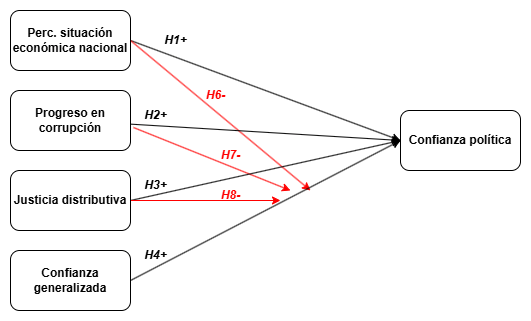
\includegraphics[width=0.8\linewidth,]{IPO/output/graphs/hipotesis_tesis} 

}

\caption{Esquema de presentación de hipótesis. Se omite la hipótesis 5. Fuente: Elaboración propia.}\label{fig:grafico-1}
\end{figure}

\chapter{Metodología}\label{metodologuxeda}

\section{Datos}\label{datos}

En específico, se trabajó sobre datos secundarios a partir de indicadores que serán extraídos de la encuesta Latinobarómetro, en su ola correspondiente al año 2023. Para el caso chileno, esta encuesta presenta una muestra de 1200 entrevistados, los cuales fueron seleccionados mediante un muestreo probabilístico en tres etapas y representan al 100\% de la población adulta en el país. Estos datos fueron levantados entre el 20 de febrero y el 1 de abril del 2023 mediante entrevistas presenciales en formato cara a cara.

\section{Variables}\label{variables}

\subsection{Variable dependiente}\label{variable-dependiente}

Para medir el nivel de confianza política, se usó la siguiente pregunta: Por favor, mire esta tarjeta y dígame, para cada uno de los grupos, instituciones o personas de la lista ¿Cuánta confianza tiene usted en ellas: mucha (1), algo (2), poca (3) o ninguna (4) confianza en\ldots?. La elección de esta pregunta constituye una ventaja metodológica, debido a que no hace ninguna referencia al desempeño de las instituciones ni a quienes las ocupan, lo que nos permite asegurarnos que se están tomando como referencia las instituciones políticas en cuanto objeto político distinguible de los actores que las lideran. De la lista de instituciones que se le menciona a los encuestados, se analiza el nivel de confianza reportado en las instituciones centrales del régimen político democrático, es decir, el Congreso, el gobierno, el Poder Judicial y los partidos políticos. A partir de las respuestas de cada una de estas instituciones se construyó un índice aditivo de escala 1-10 (\(\alpha\) = 0.78) que sirve de variable para medir la confianza política como una dimensión única. Lo anterior se justifica a partir del reconocimiento por gran parte de la literatura de que, a nivel empírico, las actitudes expresadas frente a este conjunto de instituciones están determinadas por la orientación general que los individuos tienen hacia el sistema político \citep{marienMeasuringPoliticalTrust2013, zmerliPoliticalTrust2022}. A su vez, se ha comprobado la pertinencia de este indicador en investigaciones previas \citep{bargstedSocialPoliticalTrust2023, zmerliIncomeInequalityDistributive2015}.

\subsection{Variables independientes}\label{variables-independientes}

Para estudiar la pertinencia de las explicaciones sobre las causas de la confianza política mencionadas en el apartado de marco teórico, se seleccionó un indicador para cada una. En lo que respecta a la percepción de la situación económica del país, se construyó un índice sumativo de escala 1-10 (\(\alpha\) = 0.76) a partir de las respuestas a tres preguntas: 1) ¿Cómo calificaría en general la situación económica actual del país?; 2) ¿Considera Ud. que la situación económica actual del país está mucho mejor, un poco mejor, igual, un poco peor, o mucho peor que hace doce meses?; 3) ¿Y en los próximos doce meses cree Ud. que, en general, la situación económica del país será mucho mejor, un poco mejor, igual, un poco peor, o mucho peor que ahora? La primera de estas comprende los valores desde el 1 (Muy buena) hasta el 5 (Muy mala). Por otro lado, la segunda y la tercera incluyen el mismo rango de valores pero cambia el fraseo, el cual va desde Mucho mejor (1) a Mucho peor (5). A partir de este indicador, se obtiene un panorama más completo de la percepción del individuo a este respecto, debido a que no se limita a conocer únicamente su opinión sobre el presente económico nacional sino que también la comparación que hace con el pasado y sus proyecciones a futuro \citep{saldanazunigaConfianzaInstitucionesPoliticas2019}.

En cuanto a la percepción de la corrupción, se hizo uso de la pregunta ¿Cuánto cree Ud. que se ha progresado en reducir la corrupción en las instituciones del Estado en estos últimos 2 años?, la cual incluye como categorías de respuesta valores del 1 (Mucho) al 4 (Nada). De esta forma, se podrá obtener información de la evaluación que los ciudadanos llevan a cabo sobre la eficiencia de las instituciones en combatir la corrupción. A su vez, este indicador ha sido utilizado con éxito en investigaciones similares \citep{andrianiInstitutionalTrustCorruption2021}. Por otro lado, en lo que respecta a la percepción de la desigualdad de ingresos se ocupó la pregunta ¿Cuán justa cree Ud. que es la distribución del ingreso en Chile?, la cual comprende valores del 1 (Justa) al 4 (Muy injusta). Este indicador se condice con los estudios sobre percepción de desigualdad y confianza política \citep{leeEconomicPerformanceIncome2020, wuIncomeInequalityDistributive2019, zmerliIncomeInequalityDistributive2015}. Para efectos del análisis, ambos indicadores fueron transformados en variables \emph{dummy}. En el caso del primero se agruparon, por un lado, las categorías ``Mucho'' y ``Algo'' y, por el otro lado, las de ``Poco'' y ``Nada''. A su vez, en lo que respecta al segundo se agruparon en una categoría las respuestas ``Muy Justa'' y ``Justa'' y en otra las de ``Injusta'' Y ``Muy injusta''. En ambas recodificaciones se ordenaron las categorías de respuesta de manera tal que el valor ``1'' indique una percepción negativa del desempeño institucional en cada uno de estos ámbitos.

Por último, para medir la confianza generalizada se utilizó la siguiente pregunta: Hablando en general, ¿Diría Ud. que se puede confiar en la mayoría de las personas o que uno nunca es lo suficientemente cuidadoso en el trato con los demás? Esta, a su vez, ofrece las siguientes dos categorías de respuesta: 1) Se puede confiar en la mayoría de las personas; 2) No se puede confiar en la mayoría de las personas. Al igual que las últimas dos, esta variable se recodificó para que adoptara valores ``1'' y ``0'', en los que la puntuación ``1'' expresa confianza generalizada y la puntuación ``0'' indica falta de este atributo. Este indicador, difundido originalmente por Rosenberg \citeyearpar{rosenbergMisanthropyPoliticalIdeology1956}, es el más utilizado por las encuestas para medir la confianza generalizada, y por tanto es adoptado por la mayoría de las investigaciones que ocupan este concepto \citep{andrianiInstitutionalTrustCorruption2021, garcia-sanchezEconomicInequalityUnfairness2025a, mattesSocialPoliticalTrust2018, newtonThreeFormsTrust2011, oskarssonGeneralizedTrustPolitical2010}. Aunque algunos investigadores ponen en duda su funcionalidad debido a que el significado de la frase ``la mayoría de las personas'' se puede prestar para interpretaciones distintas según el individuo \citep{justwanMeasuringSocialTrust2018}, se afirma su pertinencia en cuanto la amplitud en su fraseo permite asumir que lo que se está midiendo es la confianza en los desconocidos \citep{oskarssonGeneralizedTrustPolitical2010, uslanerMoralFoundationsTrust2002}, lo que se encuentra en concordancia con la definición de confianza generalizada adoptada en este estudio.

\subsection{Variables de control}\label{variables-de-control}

Además de los indicadores ya mencionados, se incluyeron en el análisis un conjunto de variables sociodemográficas a modo de variables de control. Estas son: sexo, edad, nivel educacional, estatus social subjetivo y afiliación religiosa.

\section{Métodos}\label{muxe9todos}

Una vez procesada la información contenida en la encuesta Latinobarómetro, se llevaron a cabo las mediciones pertinentes a los objetivos de la investigación. Para esto, en primer lugar, se calcularon una serie de estadísticos descriptivos sobre las variables principales del estudio con el objetivo de presentar un panorama general sobre el estado de estas en la población chilena. En segundo lugar, en orden de comprobar las hipótesis esgrimidas en el apartado anterior, se construyeron modelos de regresión múltiple (MCO). Se eligió esta técnica de investigación en cuanto permite estimar la intensidad y la significación estadística de las relaciones formuladas, así como controlar por el efecto de otras variables, reduciendo al máximo posible el error de en la estimación. Con los datos que proporcionan los modelos, es posible llevar a cabo inferencias respecto a la influencia del desempeño institucional y de la confianza generalizada en la confianza política, así como explorar de qué forma interactúan estos dos posibles determinantes.

\chapter{Análisis}\label{anuxe1lisis}

\section{Análisis descriptivo}\label{anuxe1lisis-descriptivo}

\label{tab:tabla-1}Estadísticas descriptivas

\textbf{Variable}

\textbf{N = 1,061}

\textbf{Indice de confianza política}

3.54 (1.89)

\textbf{Indice de percepción de la situación económica}

5.04 (1.83)

\textbf{Progreso en reducir la corrupción política}

Mucho/Algo

271.0 (25.5\%)

Poco/Nada

790.0 (74.5\%)

\textbf{Justicia en la distribución de ingresos}

Muy justa/Justa

48.0 (4.5\%)

Injusta/Muy injusta

1,013.0 (95.5\%)

\textbf{Confianza generalizada}

Uno nunca es lo suficientemente cuidadoso en el trato con los demás

874.0 (82.4\%)

Se puede confiar en la mayoría de las personas

187.0 (17.6\%)

\textbf{Sexo}

Hombre

514.0 (48.4\%)

Mujer

547.0 (51.6\%)

\textbf{Grupo etario}

16-25

157.0 (14.8\%)

26-40

303.0 (28.6\%)

41-60

397.0 (37.4\%)

61 y más

204.0 (19.2\%)

\textbf{Religión}

Ninguna/Ateo/Agnóstico

358.0 (33.7\%)

Católica

585.0 (55.1\%)

No católica

118.0 (11.1\%)

\textbf{Nivel educacional}

Sin universitario completo

873.0 (82.3\%)

Con universitario completo

188.0 (17.7\%)

\textbf{Estatus social subjetivo}

Clase Baja/Media baja

535.0 (50.4\%)

Clase Media

480.0 (45.2\%)

Clase Media alta/Alta

46.0 (4.3\%)

{\emph{Notas:}}

Media (Desviación estándar) para variables continuas; n (\%) para categóricas.

Fuente: Elaboración propia en base a Latinobarómetro 2023.

En la Tabla \ref{tab:tabla-1} se presentan las estadísticas descriptivas de las variables incluidas en el análisis. En esta, se observa que los ciudadanos chilenos poseen un bajo nivel de confianza en sus instituciones políticas, obteniendo un promedio de 3.54 (\emph{de} = 1.89) en el índice de confianza política. De esta forma, los datos analizados mantienen la tendencia mostrada por anteriores estudios a este respecto. A su vez, se evidencia una evaluación negativa del desempeño de las instituciones estatales en el combate de la corrupción, con solo un 26\% de personas que indican que se ha progresado a este respecto en los últimos dos años. Lo anterior se profundiza en lo que respecta a la desigualdad de ingresos, con solo un 5\% individuos que califica como justa la distribución de ingresos en el país. Esta evaluación mejora cuando se examina el índice de percepción de situación económica, en el cual la población obtuvo como promedio un valor de 5.04 (\emph{de} = 1.83). Por ultimo, destaca el bajo nivel de confianza generalizada evidenciado, con solo un 18\% de sujetos que declaran poder confiar en la mayoría de las personas.

\begin{figure}[!ht]

{\centering 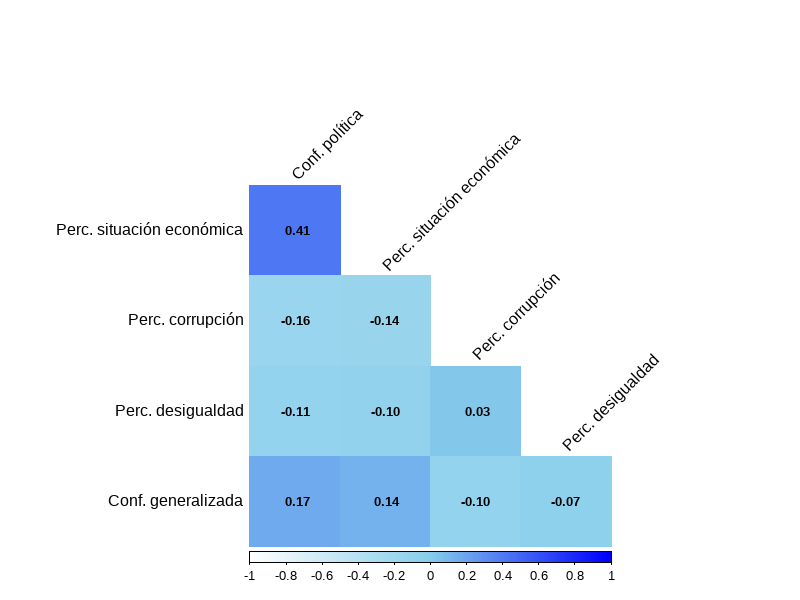
\includegraphics[width=1\linewidth,]{IPO/output/graphs/corrplot} 

}

\caption{Matriz de correlaciones entre las variables principales del estudio. Fuente: Elaboración propia en base a Latinobarometro 2023.}\label{fig:grafico-2}
\end{figure}

Por otro lado, en la Figura \ref{fig:grafico-2} se expone una matriz de correlaciones en la que se evidencia el grado de asociación de las distintas variables principales entre sí. En esta, se observa que todas las variables independientes se asocian positivamente con la variable de confianza política, aunque con distinto grado de intensidad. En este sentido, la percepción de situación económica de los individuos se asocia moderadamente con este indicador (\emph{r} = 0.41, p \textless{} 0.001). Por el contrario, el resto de variables muestran un grado bajo de asociación, siendo la percepción de desigualdad de ingresos la que en menor grado se relaciona con la confianza política (\emph{r} = 0.11, p \textless{} 0.001), seguido por la percepción de corrupción (\emph{r} = 0.16, p \textless{} 0.01) y, por último, la confianza generalizada (\emph{r} = 0.17, p \textless{} 0.001).

\section{Modelos}\label{modelos}

\label{tab:tabla-regresiones} Resultados modelos de regresión lineal MCO

~

Modelo 1

Modelo 2

Modelo 3

Modelo 4

Predictores

\textbf{\(\beta\)}

\textbf{se}

\textbf{\(\beta\)}

\textbf{se}

\textbf{\(\beta\)}

\textbf{se}

\textbf{\(\beta\)}

\textbf{se}

Intercepto

2.45 ***

0.32

2.34 ***

0.32

1.90 ***

0.36

2.09 ***

0.41

Perc situación económica

0.40 ***

0.03

0.39 ***

0.03

0.39 ***

0.03

0.38 ***

0.03

Perc desigualdad de ingresos

-0.63 *

0.25

-0.58 *

0.25

-0.50 *

0.25

-0.63 *

0.30

Perc corrupción

-0.44 ***

0.12

-0.40 ***

0.12

-0.38 **

0.12

-0.40 **

0.14

Conf.generalizada

0.53 ***

0.14

0.49 ***

0.14

-0.27

0.75

Sexo

0.17

0.10

0.17

0.11

Grupo etario 26-40

0.01

0.17

0.01

0.17

Grupo etario: 41-60

0.11

0.16

0.11

0.17

Grupo etario: \textgreater{} 61

0.02

0.18

0.02

0.18

Religión: Católico

0.20

0.12

0.19

0.12

Religión: No católico

-0.18

0.18

-0.19

0.18

Universitario

0.14

0.15

0.14

0.15

ESS: Clase Media

0.22 *

0.11

0.22 *

0.11

ESS: Clase Alta/Media alta

0.51

0.28

0.51

0.28

Perc situación económica X Conf generalizada

0.05

0.08

Perc desigualdad de ingresos X Conf generalizada

0.46

0.57

Perc corrupción X Conf generalizada

0.06

0.29

Observations

1061

1061

1061

1061

R2 / R2 adjusted

0.185 / 0.183

0.196 / 0.193

0.212 / 0.203

0.213 / 0.201

\begin{itemize}
\tightlist
\item
  p\textless0.05~~~** p\textless0.01~~~*** p\textless0.001
\end{itemize}

Fuente: Elaboración propia en base a Latinobarómetro 2023. N = 1,200

Cómo se puede observar en la Tabla \ref{tab:tabla-regresiones}, se construyeron un total de cuatro modelos de regresión lineal siguiendo una estrategia incremental, en la cual se van incorporando nuevos términos a la regresión para comprobar si se mantienen los efectos percibidos. Siguiendo esta lógica, el Modelo 1 se calculó solo con las variables de percepción del desempeño. Luego, en los Modelos 2 y 3 se introdujeron, respectivamente, la variable de confianza generalizada y las variables de control. Por último, en el Modelo 4 se añadieron los términos de interacción.

Examinando los resultados de los primeros dos modelos, se observa que tanto las variables de percepción del desempeño como la de confianza generalizada presentan efectos estadisticamente significativos que se mantienen en ambas estimaciones. Por un lado, en lo que respecta a las primeras (Modelo 1) se advierte que aquellos individuos que poseen una percepción más positiva de la situación económica del país presentan, en promedio, 0.40 puntos adicionales (\emph{se} = 0.03, p \textless{} 0.001) en el índice de confianza política. En contraste, los ciudadanos que declaran tener una percepción negativa del progreso obtenido en combatir la corrupción en las instituciones del Estado exhiben valores promedio más bajos de confianza política (\(\beta\) = -0.44; \emph{se} = 0.12, p \textless{} 0.001), al igual que aquellos que califican como injusta o muy injusta la distribución del ingreso en el país (\(\beta\) = -0.63, \emph{se} = 0.25, p \textless{} 0.05). Por otro lado, se encuentra una relación positiva entre la confianza generalizada y la variable dependiente (Modelo 2), la cual se traduce en que aquellas personas que señalan confiar en la mayoría de las personas reportan, en promedio, un mayor grado de confianza en las instituciones políticas (\(\beta\) = 0.53, \emph{se} = 0.14, p \textless{} 0.001).

\begin{figure}[!ht]

{\centering 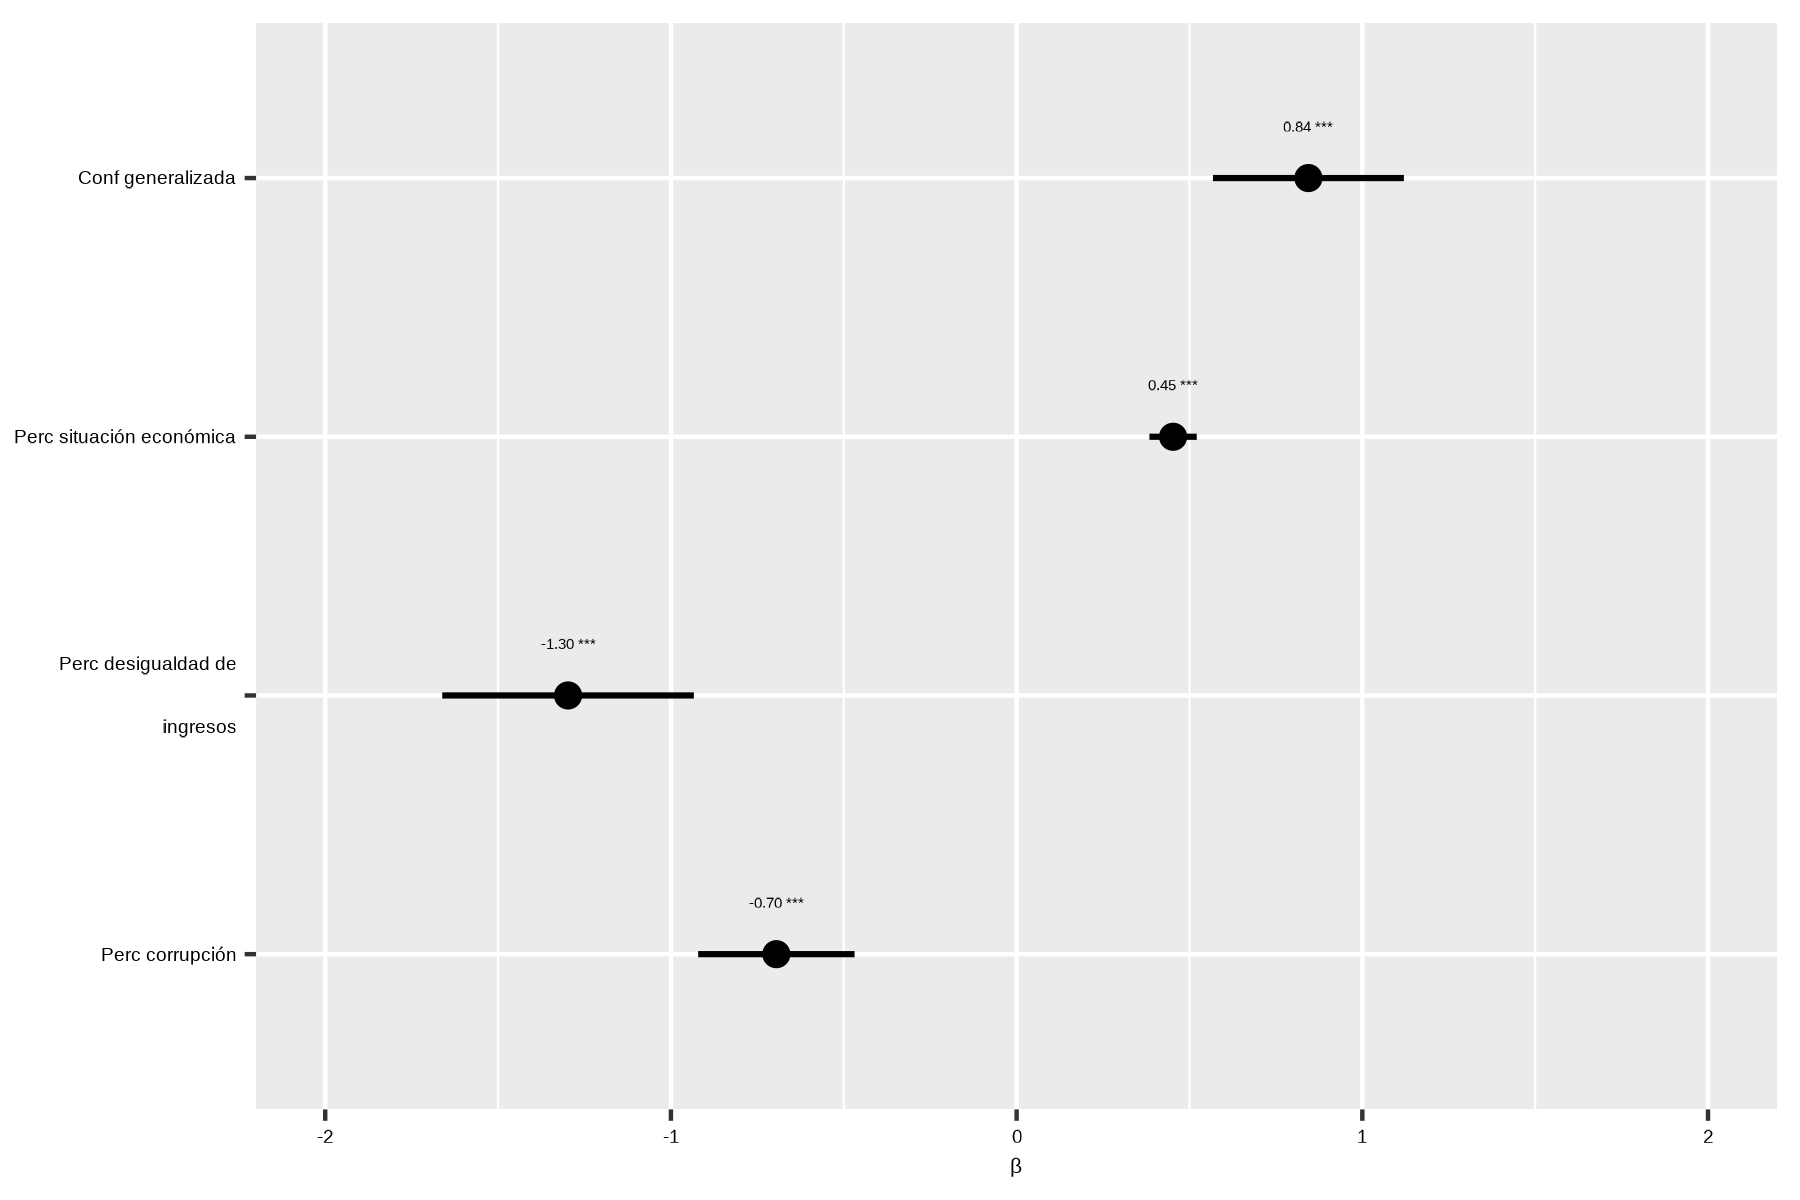
\includegraphics[width=1\linewidth,]{IPO/output/graphs/coeficientes} 

}

\caption{Comparación coeficientes de regresión Modelo 3. Fuente: Elaboración propia en base a Latinobarómetro 2023.}\label{fig:grafico-3}
\end{figure}

Al comparar las estimaciones de estos dos modelo con las del Modelo 3, se observa que la variable que se mantiene más estable a lo largo de las distintas mediciones es la de percepción de situación económica, la cual disminuye solamente en dos unidades. Respecto a las otras, la percepción de desigualdad de ingresos es la que presenta un mayor cambio, en cuanto su efecto disminuye en 10 unidades, seguido de la percepción de corrupción cuyo efecto disminuye en 6 unidades. Por último, el efecto de la confianza generalizada en la confianza política se reduce en 3 unidades. No obstante los cambios, estas variables se mantienen estadisticamente significativas, de manera tal que es posible aceptar las hipótesis \emph{H1}, \emph{H2}, \emph{H3} y \emph{H4}. En contraste, al comparar entre sí la magnitud del efecto que las distintas variables dependientes tienen sobre el índice de confianza política (véase Figura \ref{fig:grafico-3}), se evidencia que los resultados no permiten aceptar la Hipótesis \emph{H5}. Lo anterior debido a que el efecto de la confianza generalizada sobre la confianza política es mayor que el de algunas variables de percepción del desempeño político, siendo solo superado por el efecto de la percepción de la desigualdad de ingresos.

Por último, se presentan los resultados del Modelo 4, que incluye los efectos de interacción entre la confianza generalizada y cada una de las variables de percepción del desempeño. En esta, se evidencia que el efecto de la percepción de la desigualdad de ingresos se atenúa cuando los individuos confían en la mayoría de las personas (\(\beta\) = 0.44, \emph{se} = 0.57, p \textgreater{} 0.5). En lo que respecta a la percepción de la situación económica y de la desigualdad de ingresos, ambas presentan efectos de interacción con la confianza generalizada muy bajos (respectivamente: \(\beta\) = 0.06, \emph{se} = 0.08, p \textgreater{} 0.5; \(\beta\) = 0.05, \emph{se} 0.29, p \textgreater{} 0.05). Pese a lo anterior, es necesario examinar con cautela estos resultados debido al gran error estándar (\emph{se}, por sus siglas en inglés) que presenta cada una de las variables, lo que indica que estas estimaciones son poco confiables desde el punto de vista estadístico. A su vez, ninguno de los efectos de interacción estimados es significativo. Todo lo anterior obliga a rechazar las hipótesis \emph{H6}, \emph{H7} y \emph{H8}.

\chapter{Conclusiones}\label{conclusiones}

\chapter*{Bibliografía}\label{bibliografuxeda}
\addcontentsline{toc}{chapter}{Bibliografía}

% %%%%%%%%%%%%%%%%%%%%%%%%%%%%%%%%%%%%%%%%%%%%%%%%%
% %%% Bibliography                              %%%
% %%%%%%%%%%%%%%%%%%%%%%%%%%%%%%%%%%%%%%%%%%%%%%%%%
% \addtocontents{toc}{\vspace{.5\baselineskip}}
% \cleardoublepage
% \phantomsection
% \addcontentsline{toc}{chapter}{\protect\numberline{}{Bibliography}}
\bibliography{tesis}

%% All books from our library (SfS) are already in a BiBTeX file
%% (Assbib). You can use Assbib combined with your personal BiBTeX file:
%% \bibliography{Myreferences,Assbib}. Of course, this will only work on
%% the computers at SfS, unless you copy the Assbib file
%%  --> /u/sfs/bib/Assbib.bib



\end{document}
